We perform experiments on a combination of publicly-available image datasets -- Coloured MNIST
(following a similar data-generation process to \citet{KehBarThoQua20}) and CelebA
\citep{liu2015celeba}.
%and Chest-Xray8 \citep{wang2017chestx}. 
%
We report the \texttt{Robust Accuracy} -- the minimum accuracy over the subgroups -- for all
datasets but the Chest-Xray8 dataset. 
%
For this dataset, we instead report \texttt{Robust TPR} -- analogously, the minimum \ac{TPR} over the
subgroups -- as the primary metric given the emphasis on positive classifications in medical
contexts. 
%
Additional plots showing the Accuracy, Positive Rate, \ac{TPR}, and \ac{TNR} ratios can be found in
Appendix~\ref{sec:additional-metrics}.

% To validate the step of constructing the perfect bags,
We compare the performance of our disentangling model when paired with each of three different bag
balancing methods: 1) with clustering via rank statistics (\texttt{Clustering}); 2) without
balancing, when the deployment set $\gD^{dep}$ is used as is (\texttt{No Balancing}); 3) with
balancing using the ground-truth class and subgroup labels (\texttt{Oracle Bag}) that would in
practice be unobservable; this provides insight into the performance under ideal conditions and how
sensitive the method is to bag imbalance.
 
\subsection{Coloured MNIST}\label{ssec:cmnist_exp}
%
\begin{figure*}[t]
  \centering
  \begin{subfigure}[b]{\textwidth}
  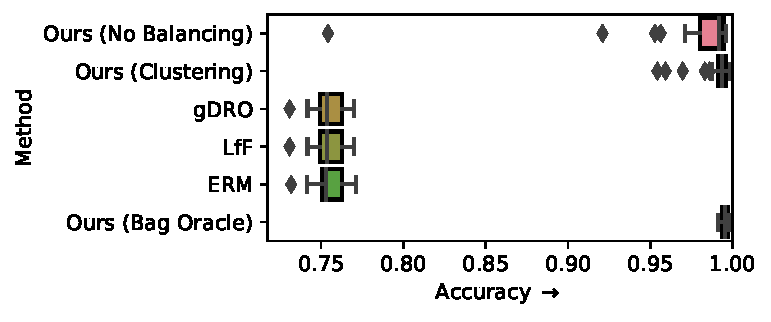
\includegraphics[width=0.49\textwidth]{supmatch/figures/cmnist/subgroup_bias/cmnist_2v4_partial_acc.pdf}
  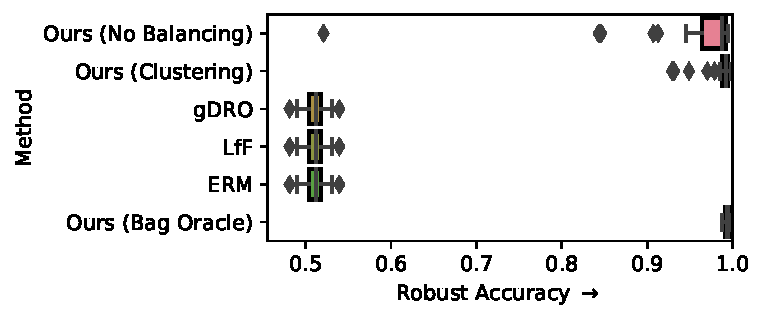
\includegraphics[width=0.49\textwidth]{supmatch/figures/cmnist/subgroup_bias/cmnist_2v4_partial_acc-min.pdf}
%   \includegraphics[width=\columnwidth]{figures/cmnist_2v4_partial_tpr.pdf}
%   \includegraphics[width=\columnwidth]{figures/cmnist_2v4_partial_tnr.pdf}
  \caption{
    Results for the \emph{subgroup-bias} scenario where {\color{purple}purple} fours constitute the missing source.
    %
    The clustering accuracy for \texttt{Ours (No Balancing)} was 96\% $\pm$ 6\%.
    %
    Our method consistently outperforms the baselines, which fare no better than random on the subgroup with the missing source. 
    %
    As we would expect, the median and IQR of our method are positively- and negative- correlated, respectively, with how well the bags of the deployment set are balanced, with \texttt{Ours (Bag Oracle)} providing an upper bound for this.
    %
    Indeed, in one case \texttt{Ours (No Balancing)} failed to outperform the baselines, yet through
    clustering the worst-case \texttt{Robust Accuracy} is limited to within the $95\%$ region.
  }%
  \label{fig:cmnist-2v4-partial}
% \end{figure*}
% \begin{subfigure}
  \end{subfigure}
  
  \begin{subfigure}[b]{\textwidth}
  \centering
  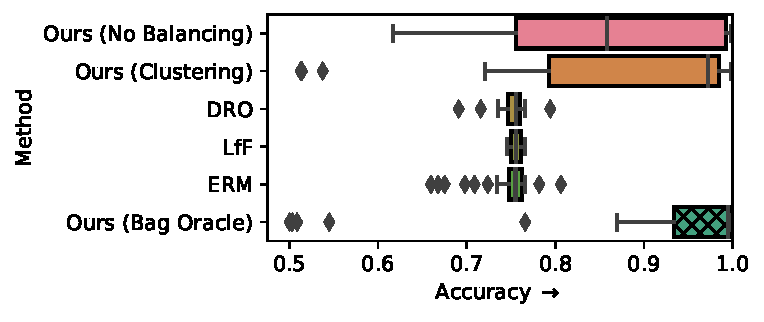
\includegraphics[width=0.49\textwidth]{supmatch/figures/cmnist/missing_subgroup/cmnist_2v4_miss_s_acc.pdf}
  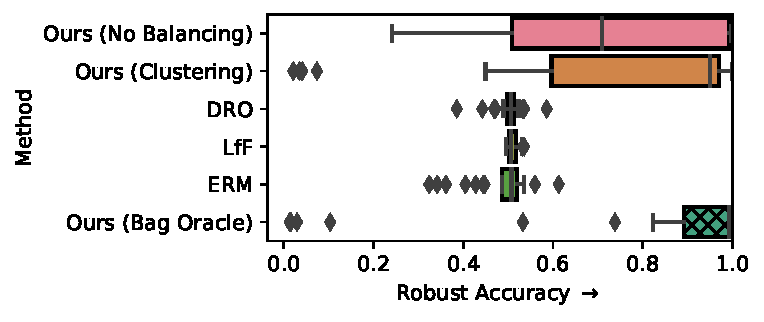
\includegraphics[width=0.49\textwidth]{supmatch/figures/cmnist/missing_subgroup/cmnist_2v4_miss_s_acc-min.pdf}
%   \includegraphics[width=\columnwidth]{supmatch/figures/cmnist_2v4_miss_s_alt_tpr.pdf}
%   \includegraphics[width=\columnwidth]{supmatch/figures/cmnist_2v4_miss_s_alt_tnr.pdf}
  \caption{
    Results for the \emph{missing-subgroup scenario} where {\color{purple}purple} digits constitute the missing subgroup.
    %
    The clustering accuracy for \texttt{Our (No Balancing)} was 88\% $\pm$ 5\%. 
    This scenario is significantly more difficult to solve than the subgroup-bias as there is insufficient inductive bias in the labels and the deployment set for the support matching to be well-posed. 
    %
    This is reflected in the high variance of our method, variance, however, which can be drastically reduced by improving the quality of balancing.
    %
    Nevertheless, all variants of our method perform significantly better than the baselines in terms of the median \texttt{Robust Accuracy}, and the rate at which they produce degenerate solutions (marked by performance worse than \texttt{ERM}'s) relatively low.
    %
  }%
  \label{fig:cmnist-2v4-miss-s}
  \end{subfigure}
  \caption{
  Results for two-digit Colored MNIST for two different scenarios (subgroup bias (Top) and missing subgroup (Bottom)) in the form of box plots of the \texttt{Robust Accuracy} (the minimum accuracy computed over the subgroups) over \textbf{30 repeats}.
  }
\end{figure*}

%
Appendix~\ref{sec:dataset-construction} provides description of the dataset and the settings used
for \( D^{dep} \) and \( D^{tr} \). 
%
Each source is then a combination of digit-class (class label) and colour (subgroup label). 
%
We begin by considering a binary, 2-digit/2-colour, variant of the dataset with $\gY = \{2, 4\}$
and $\gS = \{\text{\color{green}green}, \text{\color{purple}purple}\}$.
(Appendix~\ref{ssec:3-digit-3-color} provides results for 3-digit/3-colour variant.) 
%
For this variant we explore both the SB (subgroup bias) setting and a more extreme \emph{missing
subgroup} setting.
%
To simulate the SB setting, we set \(\gS^{tr}_{ Y=4 }=\{\text{\color{green}{green}}\}\). 
%
In the \emph{missing subgroup} setting, $S=\text{\color{purple}{purple}}$ is missing from
\(\gS^{tr}_{ Y=2 }\) as well, so that all classes only have support in
\(\{\text{\color{green}{green}}\}\).
%
However, for this scenario, the disentangling procedure has more than one possible solution --
apart from the natural solution, it is also possible to consider ($Y=2$,
$S=\text{\color{green}{green}}$) and ($Y=4$, $S=\text{\color{purple}{purple}}$) as forming one
factor in the disentangling, with the other factor comprising the two remaining
$s$-$y$-combinations.
%
Such an ``unnatural'' disentangling (spanning digit class \emph{and} colour) is avoided only by the
tendency of neural networks to prefer simpler solutions (Occam's razor) and in general we cannot
guarantee that this pathological case be avoided based only on the information provided by the
training labels and deployment set.

To establish the effectiveness of our method, we compare against four baselines.
%
The first is \texttt{ERM}, a classifier trained with cross-entropy loss on this data; the second is
\texttt{DRO} \citep{HasSriNamLia18}, which functions without subgroup labels by minimising the
worst-case training loss over all possible groups that are above a certain minimum size; the third
is \texttt{gDRO} \citep{sagawa2019distributionally}, which minimises the worst-case training loss
over predefined subgroups but is only applicable when $|\gS^{tr}| > 1$; the fourth is \texttt{LfF}
\citep{NamChaAhnLeeetal20} which reweights the cross-entropy loss using the predictions of a
purposely-biased sister network.
%
For fair comparison, the training set is balanced according to the rules defined in
\S\ref{sec:sm-adversarialsm} for all baselines.

Fig.~\ref{fig:cmnist-2v4-partial} shows the results for the SB setting. 
%
We see that the performance of our method directly correlates with how balanced the bags are, with
the ranking of the different balancing methods being \texttt{Oracle} $>$ \texttt{Clustering}$>$
\texttt{No Balancing}. 
%
Even without balancing, our method greatly outperforms the baselines, which all perform similarly.

Fig.~\ref{fig:cmnist-2v4-miss-s} shows that the problem of \emph{missing subgroups} is harder to
solve.
%
For all balancing strategies, the IQR is significantly higher than observed in the SB setting, with
the latter also giving rise to a large number of extreme outliers. 
%
The median, however, remains high, indicative of a ``hit-or-miss'' aspect to the method, albeit
with the number of hits far outweighing the misses. 
%
Visualisations of the reconstructions (Appendix~\ref{sec:qual-results})
suggest that the extreme outliers correspond to the degenerate solution mentioned above.
% with $z$ zeroed-out suggests that misses often mostly occurred due to the semantic information
% being concentrated in $\tilde{s}$ while $z$ is left to contain only residual information, even
% when $\tilde{s}$ was set to be one-dimensional and binarized. 
%
% We leave it to future work to explore how to better obviate such degeneracies.

% \begin{figure}[tbp]
%   \centering
%    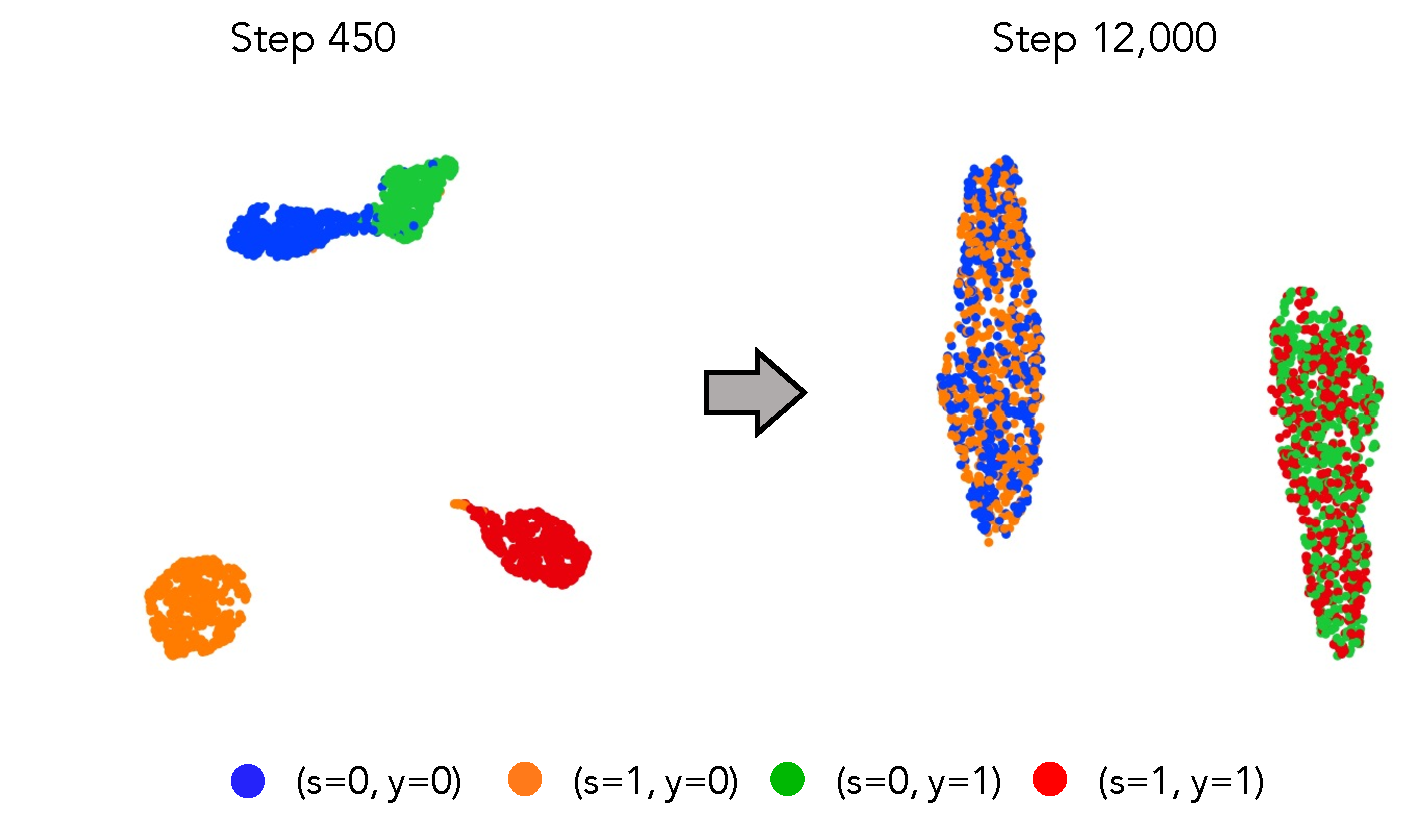
\includegraphics[width=0.6\columnwidth]{supmatch/figures/illustrations/umap_viz.pdf}
%   \caption{%
%     UMAP visualisations of the representations learned by the debiaser for the Colored MNIST
%     dataset. \textbf{Left}: After 450 training-steps each source forms a distinct cluster.
%     \textbf{Right}: After 12,000 training-steps sources with the same $y$-value have merged, thus
%     eliminating the spurious correlation between digit and color.
%   }%
%   \label{fig:umap}
% \end{figure}

% We visualise the learned representation -- from a successful run -- using UMAP
% \citep{mcinnes2018umap} in Fig.~\ref{fig:umap}. % Here, we see that at the beginning of training,
% all four sources are distinct, and the two sources with $s=0$ (from which one is missing in the
% training set) are closer to each other than to their respective classes. % At the end of
% training, the representations clearly separate into two clusters corresponding to the two
% classes, while the subgroups are distributed evenly therein.

\subsection{CelebA}\label{ssec:celeba_exp}
%
\begin{figure*}[t]
  \centering
  % Smiling females missing
%   \normalsize{Missing source: smiling females}\par\medskip
%  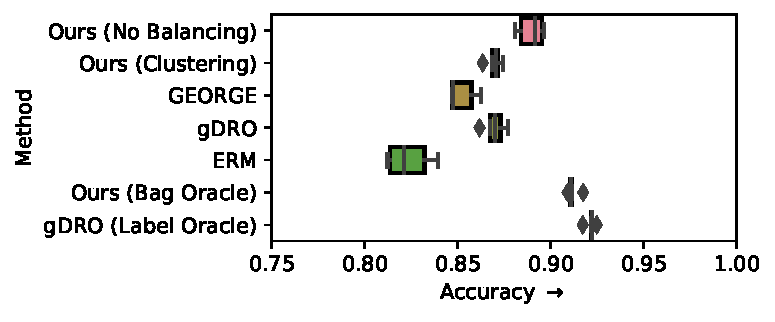
\includegraphics[width=0.49\textwidth, height=3cm]{supmatch/figures/celeba/no_smiling_females/celeba_gender_smiling_acc.pdf}
 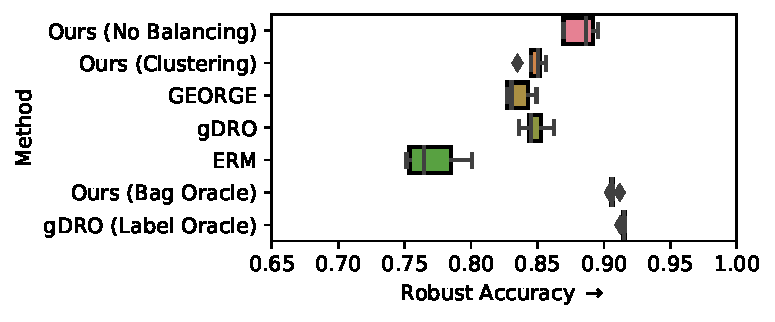
\includegraphics[width=0.49\textwidth]{supmatch/figures/celeba/no_smiling_females/celeba_gender_smiling_acc-min.pdf}
    % Smiling males missing
%   \normalsize{Missing source: smiling males}\par\medskip
%  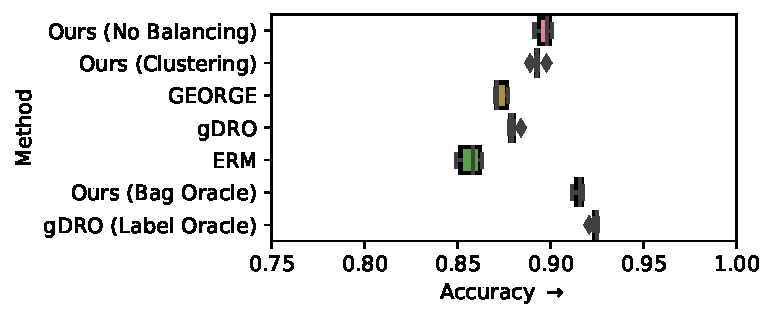
\includegraphics[width=0.49\textwidth]{supmatch/figures/celeba/no_smiling_males/celeba_gender_smiling_acc.pdf}
 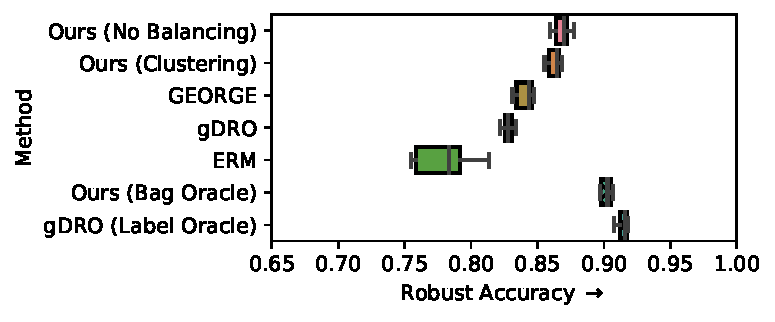
\includegraphics[width=0.49\textwidth]{supmatch/figures/celeba/no_smiling_males/celeba_gender_smiling_acc-min.pdf}
    % Unsmiling females missing
%   \normalsize{Missing source: non-smiling} females\par\medskip
%  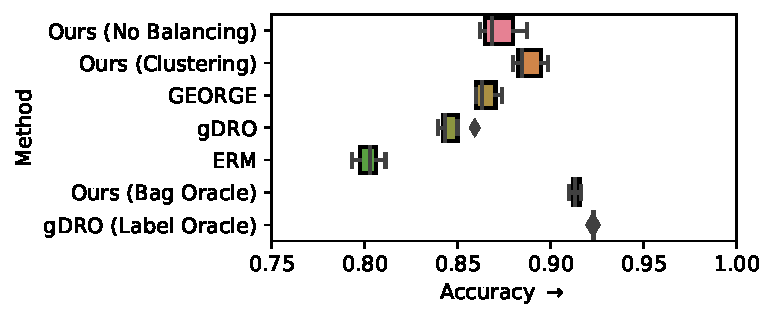
\includegraphics[width=0.49\textwidth]{supmatch/figures/celeba/no_unsmiling_females/celeba_gender_smiling_acc.pdf}
 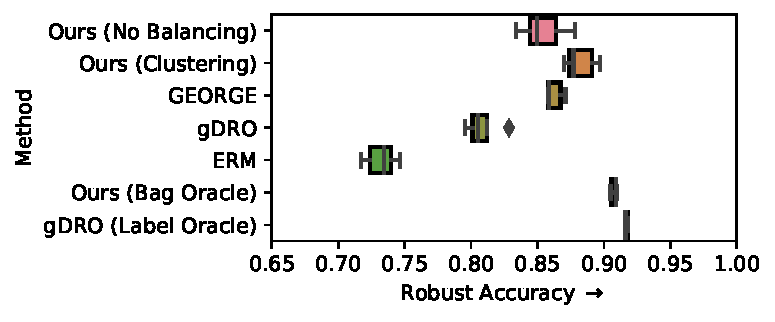
\includegraphics[width=0.49\textwidth]{supmatch/figures/celeba/no_unsmiling_females/celeba_gender_smiling_acc-min.pdf}
  % Unsmiling males missing
%   \normalsize{Missing source: non-smiling males}\par\medskip
%  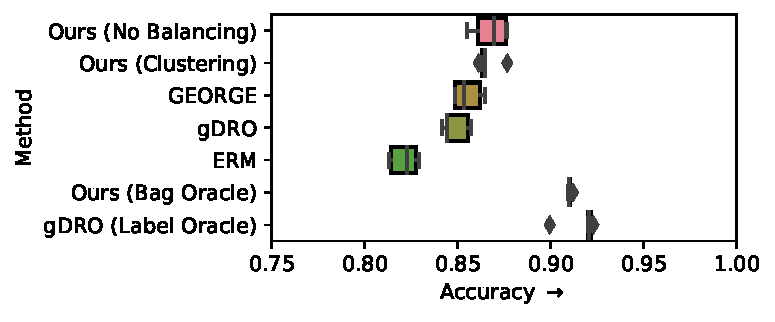
\includegraphics[width=0.49\textwidth]{supmatch/figures/celeba/no_unsmiling_males/celeba_gender_smiling_acc.pdf}
 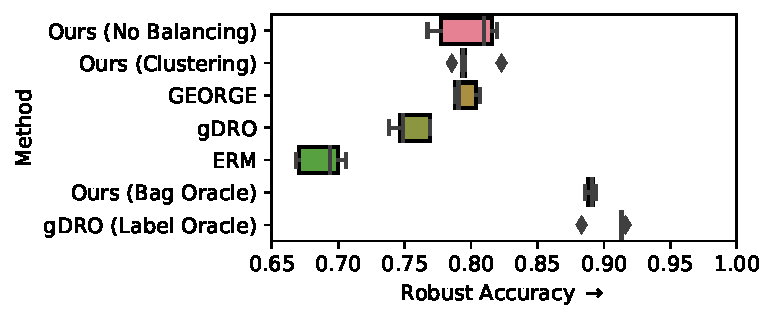
\includegraphics[width=0.49\textwidth]{supmatch/figures/celeba/no_unsmiling_males/celeba_gender_smiling_acc-min.pdf}

% compressed figures:
%   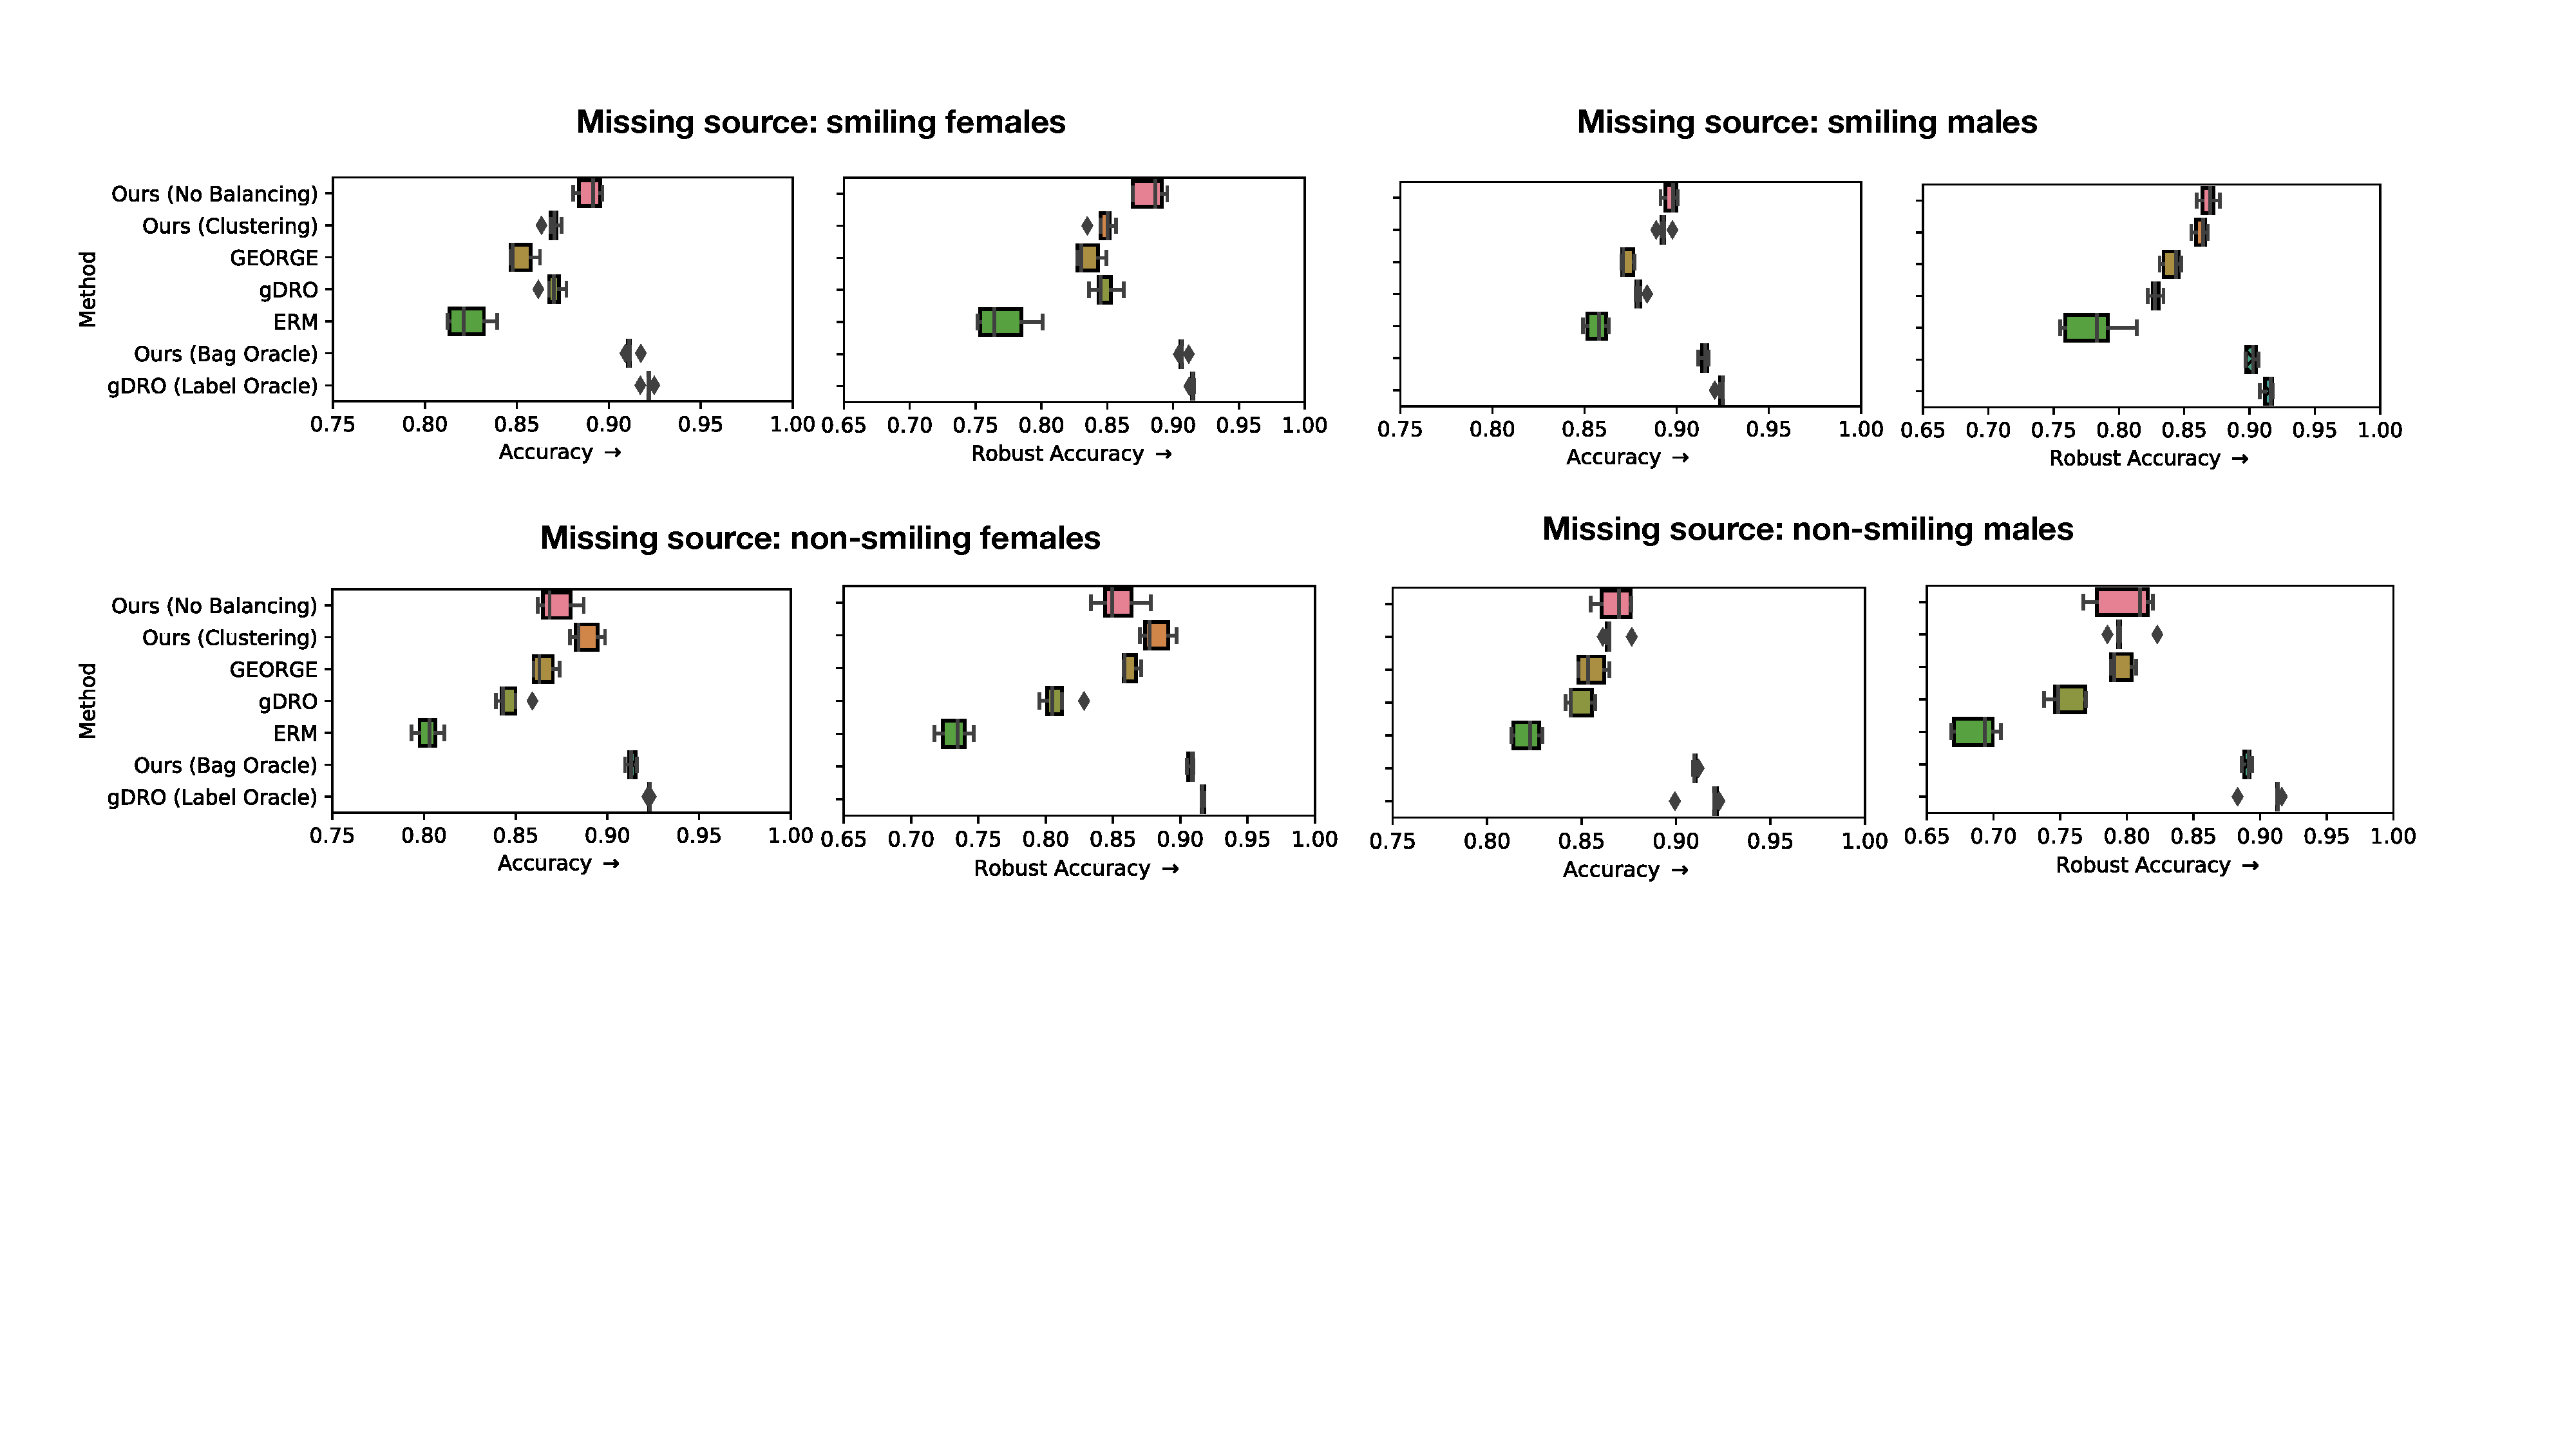
\includegraphics[width=1.0\textwidth]{supmatch/figures/celeba/CelebA2.pdf}
  \caption{
    Results from \textbf{5 repeats} for the CelebA dataset for the \emph{subgroup bias} scenario.
    The task is to predict ``smiling'' vs ``non-smiling'' and the subgroups are based on gender. 
    %
    The four sources are dropped one at a time from the training set
    (\textbf{Top Left}: smiling females; \textbf{Top Right}: smiling males; \textbf{Bottom Left}: non-smiling females;
    \textbf{Bottom Right}: non-smiling males), while the deployment set is kept fixed.
    %
    \texttt{Robust Accuracy} refers to the minimum accuracy computed over the subgroups.
    %
    Our method consistently performs on par with or outperforms \texttt{GEORGE} (which in turn outperforms \texttt{ERM}).
    %
    We note that in some of the runs, \texttt{GEORGE} performed no better than random -- these results were truncated for visibility but can be found in
    Fig.~\ref{fig:celeba-gender-smiling-full}.
    %
    % Due to poor clustering accuracy and the fact that the deployment set is naturally relatively well-balanced with respect to gender, \texttt{Ours (Clustering)} failed to improve on \texttt{Ours (No Balancing)} for all but one missing source.
    %
    Given \emph{indirect} supervision from the deployment set in the form of oracle-balancing, our method performs similarly to \texttt{gDro (Label Oracle)} that receives \emph{direct} supervision.
  }%
  \label{fig:celeba-gender-smiling}
\end{figure*}


%
To demonstrate our method generalises to real-world computer vision problems, we consider the
CelebA dataset~\citep{liu2015celeba} comprising over 200,000 images of different celebrities. The
dataset comes with per-image annotations of physical and affective attributes such as `Smiling',
`Gender', hair colour, and `Age'.
%
Since the dataset exhibits natural imbalance with respect to $\gG$, we perform no additional
sub-sampling of either the training set or the deployment set. We predict ``smiling'' as the class
label and use the binary attribute, ``gender'', as the subgroup label. Here, we consider the SB
setting but rather than just designating one missing source, we repeat our experiments with each
source being dropped in turn.
%
As before, we evaluate our method under three balancing schemes and compare with ERM and gDRO
trained on only the labelled training data.
%
We also compare with two other variants of gDRO: 1) \texttt{gDRO (Label Oracle)}, a variant that is
trained with access to the ground-truth labels of the deployment set, thus providing an upper-bound
on the downstream classification performance; 2) \texttt{GEORGE} \citep{SohDunAngGuetal20}, which
follows a two-step procedure of first clustering to obtain the labels for hidden subgroups, and
then using these labels to train a robust classifier using gDRO.
%
\citet{SohDunAngGuetal20} consider a different version of the problem (termed
\emph{hidden-stratification}) in which the class labels are known for all samples but the
subgroup-labels are missing entirely.
%
We adapt \texttt{GEORGE} to our setting by modifying the semi-supervised clustering algorithm to
predict the marginal distributions (\(P(Y|X)\) and \(P(S|X)\) instead of the joint distribution
\(P(Y, S|X)\), allowing us to propagate the class labels from \( D^{tr} \) to \( D^{dep} \) (see
Appendix~\ref{adapting_g} for details).
% Following this, gDRO is trained on the combination of the training and deployment sets, with the
% latter's labels conferred by clustering.


Fig.~\ref{fig:celeba-gender-smiling} shows the results for experiments for each missing source,
showing similar trends across all instantiations of the SB scenario. 
%
\texttt{gDRO (Label Oracle)} consistently achieves the best performance according to both metrics,
with \texttt{Our Method (Bag Oracle)} consistently coming in second. 
%
We note that while both methods use some kind of oracle, the \emph{label oracle} provides
\emph{all} class/subgroup labels to its algorithm, whereas the \emph{bag oracle} only balances the
bags. 
%
Despite the large difference in the level of supervision, the margin between the two oracle methods
is slim. 
%
We observe that clustering in many cases impairs performance which can be explained by poor
clustering of the missing source ($\sim$60\% accuracy).
%
CelebA exhibits a natural imbalance with respect to gender/smiling but not a significant one,
allowing for random sampling to yield a reasonable approximation to the desired perfect bags. 
%
We believe adjustments to the clustering algorithm -- e.g.\ using a self-supervised loss instead of
a reconstruction loss for the encoder -- could close the gap between clustering-based and
oracle-based balancing. 
%
Nonetheless, among the non-oracle methods, variants of our method
consistently match or exceed the performance of the baselines. 
%
While the plots show \texttt{GEORGE} can perform strongly in this SB scenario, we note that for
several of the missing sources, the method failed catastrophically in one out of the five runs.
%
We have cut off those data points here so as not to compromise the visibility of the other results;
the full versions of the plots can be found in Appendix~\ref{ssec:extended-results-celeba}.
%
The fact that \texttt{GEORGE} leverages both the training and deployment sets in a semi-supervised
way with clustering makes it the baseline most comparable to our method.
%
However, its performance is much more dependent on the clustering step than our method.

% %
% \subsection{Chest-Xray8}{\label{ssec:nih_exp}}
% %
% The Chest-Xray8 dataset \citep{wang2017chestx}  comprises 108,948 frontal-view X-ray images with
% weak labels -- mined automatically from radiology reports using natural language processing --
% indicating positive diagnosis of eight thoracic diseases. 
% %
% These labels are mutually inclusive and as such give rise to a multi-label classification task. 
% %
% Among the images, 24,636 are associated with one or more pathologies, while the remaining 84,312
% are derived from healthy patients.
% % Atelectasis, Cardiomegaly, Effusion, Infiltration, Mass, Nodules, Pneumonia, Pneumothorax
% To simplify the analysis, we convert the problem into one of binary classification by considering
% only he most frequently occurring pathology, ``infiltration''. 
% %
% We note that, since our method only uses the target implicitly via balancing in order to learn
% invariance to the subgroup, and this objective is balanced with the goal of maximally preserving
% information about the input, \( \gI(f(X);X) \), rather than the target directly, the resulting
% representation could be can be used for any of the targets without detriment. 
% %
% We designate ``gender'' as the subgroup label, following \citep{seyyed2020chexclusion}, and
% simulate the SB setting by dropping from the training set male patients with a positive diagnosis,
% i.e. by setting \(\gS^{tr}_{ Y=\text{infiltration} }=\{\text{female}\}\).


% \subsection{Sensitivity Analysis}\label{ssec:sensitivity}

% To assess the empirical robustness of our algorithm to noise in the bag-balancing, we conduct an
% sensitivity analysis using the Chest-Xray8 dataset. 
% %
% Using the same configuration used to collect the results from the previous section, we run our
% algorithm with the ground-truth labels used for balancing but with \( \{5\%, 10\%, \dots, 50\%\} \)
% of the labels perturbed (flipped). 
% %
% Rather than randomly perturbing the labels by sampling from the set of complementary labels --
% i.e., \( \tilde{g}_i \sim \mathrm{uniform}(\gG \setminus \{g_i\}) \), with \( g_i \) and \(
% \tilde{g}_i \) denoting the ground-truth and the perturbed labels, respectively -- which yields
% unrealistic perturbations due to the discounting the semantic relationships between groups
% (semantically similar groups are more likely to be confused by a clustering algorithm) we instead
% sample a perturbed label, $\tilde{g}_i$ from $\gG$ with probability proportional to the similarity
% between the associated (featurised) sample and the \(\tilde{g}_i\)th centroid, \(
% \phi_{\tilde{g}_i} \in \mathbb{R}^d \), with the constraint that the perturbed label does not equal
% the original one. 
% %
% This is done using features extracted by a pre-trained CLIP \citep{radford2021learning} visual
% encoder. Namely, the centroids \( \Phi \in \mathbb{R}^{|\gG| \times d} \) are computed as the
% group-conditional means of these features, over the deployment set, and their similarity with a
% given sample's features is measured using cosine similarity. 
% %
% Assuming \(L_2\)-normalised CLIP features, $\bar z_i^\text{CLIP} \in \mathbb{R}^d$, and prototypes,
% $\bar \Phi$, the sampling scheme used to generate the perturbed label, $\tilde{g}_i$, for a given
% ground-truth label, $g_i$, can be written as
% %
% \begin{align}
%   %
%   \tilde{g}_i \sim \text{Cat}(\gG, \bigtriangleup_\mathbf{w} ), \quad
%   %
%   \bigtriangleup_\mathbf{w} \triangleq  \frac{\mathbf{w}}{\sum_j \mathbf{w}_j} , \quad
%   %
%   \mathbf{w} \triangleq \text{exp}(\bar z_i^\text{CLIP} \cdot \bar \Phi \tau^{-1})
%   \odot (1 - e_{g_i}),
%   %
% \end{align}
% %
% where \( \text{Cat} \) denotes the categorical distribution with support \(\gG\) and sampling
% probabilities \( \bigtriangleup_w \), \( \tau \in \mathbb{R}^+_\ast \) denotes a temperature
% parameter modulating the sharpness of the sampling distribution, \(e_{g_i}\) denotes the one-hot
% encoding of \(g_i\), and \(\odot\) denotes the Hadamard product that is used with \(e_{g_i}\) to
% mask out the \(g_i\)th prototype and thereby enforce \( \tilde{g}_i \neq g_i \).

% which shows strong performance even without balancing.

% Now that we have them, we can discuss the results with clustering.
%
% We did not use the clustering approach for CelebA, as the attributes ``smiling'' and ``gender''
% are not the most salient; more work is needed on the clustering side to discover all semantically
% meaningful clusters.
%
% Nonetheless, our method consistently outperforms the baselines even when no balancing is applied
% Furthermore, we show qualitative results of the disentangling in fig.~\ref{fig:celeba-recons},
% and note a clear separation of subgroup-relevant information from subgroup-irrelevant
% information.
%in $g(0, f_s(x))$ and $g(f(x), 0)$, respectively.

%Furthermore, we control the \emph{number of clusters},which means all samples can get sorted into
%the right \emph{number of groups}. 
%
% Instead we use the idea of balanced dataset and sample equal amount of samples from each cluster
% to form a batch. 
  
% \textbf{Disentangled representations via adversarial autoencoders}
%We want to learn a disentanglement using a perfect dataset as the supervision signal.
%
%To achieve this, our semi-supervised disentanglement learning framework (fig.
%\ref{fig:architecture} ) maps data points into independent factors of variations such that our
%training dataset $D_{\text{tr}}$ and our deployment set $D_c$ are indistinguishable; i.e., we
%would like transform $D_{\text{tr}}$ such that the independence condition $y\perp s$ holds.
%
%However, the deployment set itself $D_c$ might not amount to a suitable target distribution in
%which the independence condition holds.
%
%The idea is to make the deployment set $D_c$ approximately perfect by balancing it according to
%the cluster IDs, forming the set $D_p$.
%
% We create disentangled representations by training four separate neural networks, which we denote
% $f$, $g$, $h$ and $l$. % We use mean squared error for the reconstruction loss, and the binary
% cross entropy error for the discriminator loss. % For a dataset with mixed-typed attributes, we
% use a combination of mean squared error and (binary) cross entropy error for the reconstruction
% loss. % We optimize the proposed model using a scheduled update scheme where we freeze the
% weights of the autoencoder and predictor modules when we update the weights of the discriminator,
% and vice versa.
%

